\documentclass[a4paper, 10pt]{article}

\usepackage[english]{babel}
\usepackage[T1]{fontenc}
\usepackage[utf8]{inputenc}
\usepackage{textcomp}
\setlength{\marginparwidth}{2cm}

\usepackage{comment}
\usepackage{todonotes}

\usepackage{amsmath}
\usepackage{amssymb}

\usepackage{enumitem}

\usepackage{xcolor}
\usepackage{graphicx}
\graphicspath{ {./img/} }

\usepackage{hyperref}
\usepackage{listings}
\usepackage{color}
\definecolor{dkgreen}{rgb}{0,0.6,0}
\definecolor{gray}{rgb}{0.5,0.5,0.5}
\definecolor{mauve}{rgb}{0.58,0,0.82}
\lstset{frame=tb,
    language=Python,
    aboveskip=3mm,
    belowskip=3mm,
    showstringspaces=false,
    columns=flexible,
    basicstyle={\small\ttfamily},
    numbers=none,
    numberstyle=\tiny\color{gray},
    keywordstyle=\color{blue},
    commentstyle=\color{dkgreen},
    stringstyle=\color{mauve},
    breaklines=true,
    breakatwhitespace=true,
    tabsize=3
}

\title{Homework Assignment N°3}
\author{BML36\\Thibault Douzon\\Rajavarman Mathivanan}
\date{September 18th, 2018}

\begin{document}
\maketitle

\pagebreak

\tableofcontents

\pagebreak

\section{Exercise 1: K-CV, under \& over-fitting}

\subsection{Part a}
To show what are under and over-fitting, we will use polynomial 
regression with different degrees on sample data. We generate 
our data points using a degree 3 polyomial and adding gaussian noise. Here is the dataset:
\\
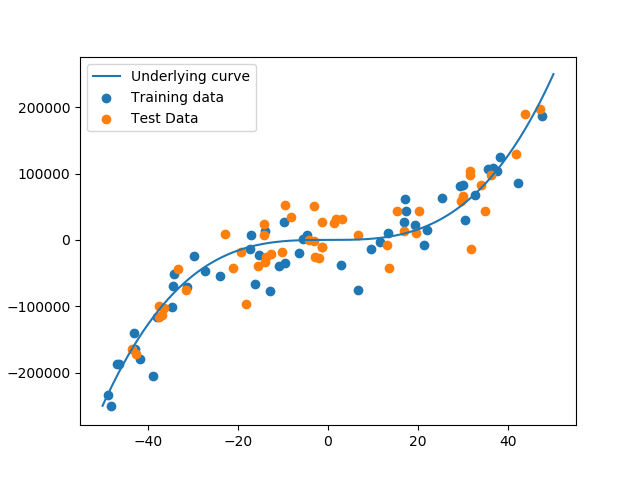
\includegraphics{ex1a_curve}
\\
Our model minimizes the sum of the squared error. Because our underlying function is a degree 3
polynomial, the best model we computed is the following, also degree 3:
\\
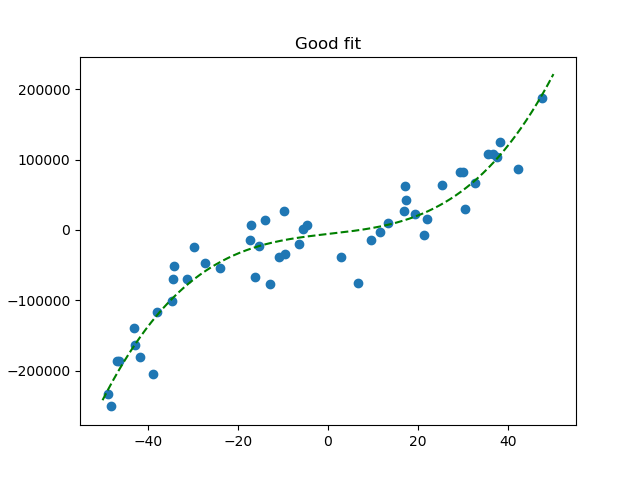
\includegraphics{ex1a_good}
\\
We can see that the green line follows accordingly our dataset, without trying to go through
every points. We can expect this model to generalize well.
\begin{itemize}[label=$\square$]
    \item Under-fitting comes when the chosen model is not complex enough
    to represent the learning data and the underlying function. 
    \\
    An under-fit model suffer from high \emph{bias} and high error on learning data.    
    We would say from such a model that it does not fit enough to the data.
    \\
    An example is our degree 0 polynomial: an horizontal line can't describe 
    correctly our underlying degree 3 polynomial:
    \\
    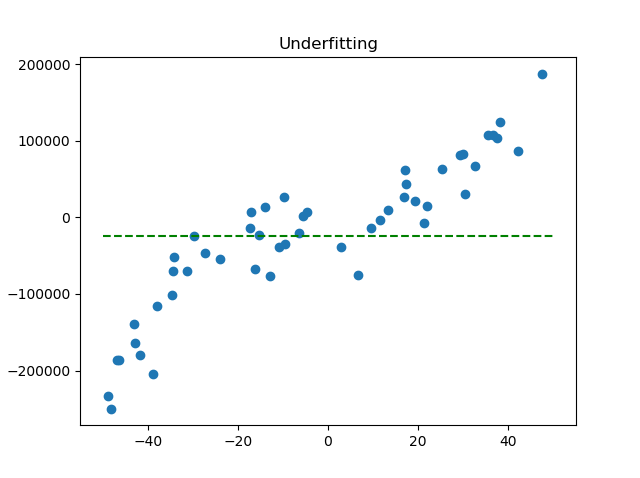
\includegraphics{ex1a_under}
    \\
    The x and y axis represent the $x$ and $y$ coordinates for our points such that
    $f(x) \approx y$.
    \\
    We can see on the previous plot that the green line is close to points in the 
    middle but makes a non negligeable error on extreme points.
    \\
    When controlling the learning with a test dataset, we know we are under-fitting when
    both the error on the training and the test data is high: our model does not describe 
    correctly the learning data and can't generalize to other data.
    
    \item Over-fitting comes when to model sticks too much to the learning data. In some sense, 
    our model tries to interpret the noise present in the learning data as if it were significant.
    \\
    An over-fit model suffer from high \emph{variance} and high error on testing data.
    \\
    An example of over-fit model is our degree 20 polynomial model:
    \\
    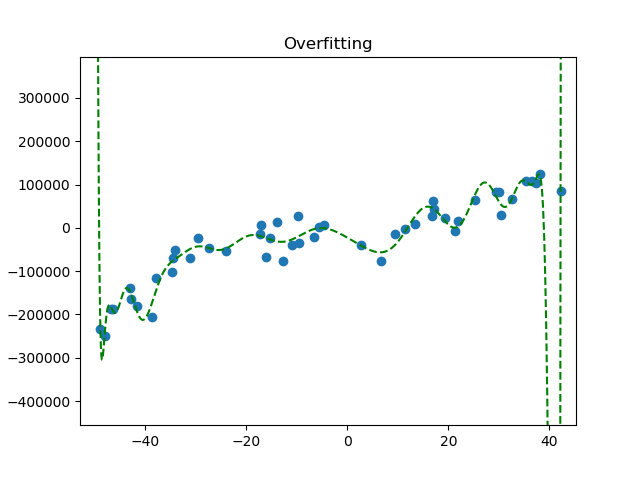
\includegraphics{ex1a_over}
    \\
    As before, this plot shows the learning data and the curve of the model.
    We can see the curve tries to pass through every points even those remote from the underlying
    curve (which suffer from high noise).
    \\ 
    Another sign of over-fitting is very high value for parameters of the model (absolute value). 
    This symptom is why we can use L1 or L2 regularization to prevent us from over-fitting.
\end{itemize}
To better see both phenomena in one figure, we can plot the error in term of the degree of our model.
If we do so for both training and testing dataset, we get the following plot:
\\
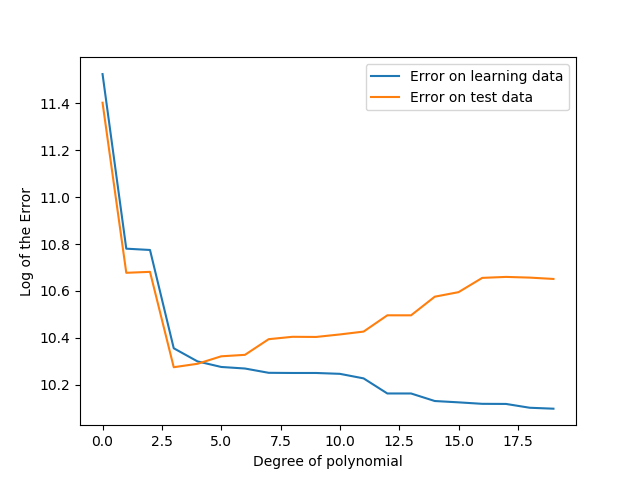
\includegraphics{ex1a_error}
\\
On this figure we can see that the error on learning data is globally always decreasing (very steeply at the beginning, then slowly)
when the complexity of the model increases. But the curve of the error on the testing data does not follows the same pattern: it first 
decreases up to some degree and then increases again. 
\\
We can divide the previous figure in two areas, one represents under-fitting and the other over-fitting. And between the 
two lays the models that may generalyze well:
\\
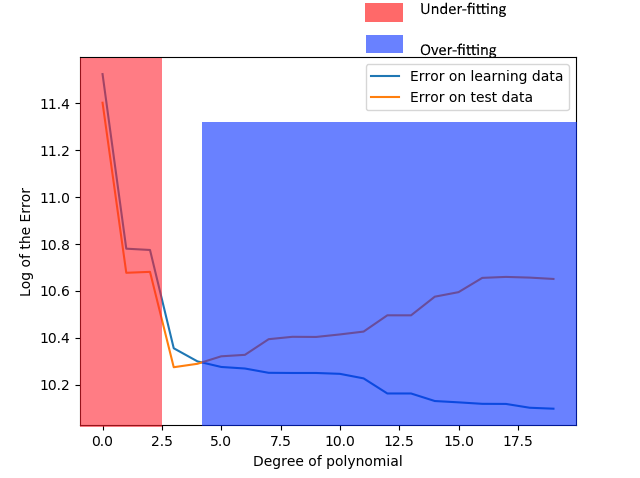
\includegraphics{ex1a_area}
\\
As we said before, in the red area both curves decrease steeply: this is the under-fitting zone.
In the blue one, error on learning data continue decreasing but slowly while error on testing data increases:
this is the over-fitting zone.

\subsection{Part b}
It is not a good idea to simply divide our dataset in training/testing and
test each model on the test set to select the best model because it could result in over-fitting
and model the noise in the test set instead of the underlying model. Especially if we 
provide more data to the learning set than to the test set: the smaller the test set,
the more noisy is our testing, and the more probable a model can fall in over-fitting.
\\
Indeed, nothing tells us the the best model on the test set will generalize well and isn't 
over-fitting the test sample also.
\\
This over-fitting on the test dataset situation could happen if we try to guess the best hyperparameters of
the model using the test set. Learning and then filtering the best hyperparameters using the test set
multiple times recursively will result in a selection of models that can overfit the test data and thus 
provide in the end an over-fit model. That's why a different set is necessary.

\subsection{Part c}
We use K-fold cross-validation because we want to use as much data as possible for training.
But keeping away test and validations sets from our training set. K-CV allows us to use the whole
dataset for training and still keep an eye on the over-fitting whereas data in the validation set will never
be used for learning.
\\
Pros: 
\begin{itemize}
    \item The whole dataset can be used for training. Very useful when we don't have many data.
    \item Can be used to determine the hyperparameters of our models: train all the
    different models with different parameters K times each and pick the best at the end
    (the one with the minimal mean of the error on the evaluation part remaining)
    \item It provides an accurate estimation of the performance of the model
    \item Offers a viable solution when training data is scarce. Doing N splits will provide a a good estimation of 
    performance.
\end{itemize}
Cons:
\begin{itemize}
    \item The learning time is increased by a factor K: if we split our dataset in 10 parts, we 
    will need 10 different trainings and thus it will last 10 times more to train.
    \item The number of folds we make is another parameter: when the dataset is small we can split in
    as many sets as the number of data, but it's too computer intensive when the dataset gets large.

\end{itemize}
\section{Exercise 2: ROC curve}
\subsection{Part a}
We can represent this situation with a table where a column represents what the model predicts (positive or negative)
and the rows represents the reality of the data. In the heading, the probability that the inequation is true is between the parenthesis
\\
\begin{center}
\begin{tabular}{ |c|c|c| }
    \hline
    \  & $x<\theta$ $\rightarrow$ ($\theta$) & $x>\theta$ $\rightarrow$ ($1-\theta$) \\
    \hline
    P & $\text{TP} = \theta \text{P}$ & $\text{FN} = (1-\theta) \text{P}$ \\
    N & $\text{FP} = \theta \text{N}$ & $\text{TN} = (1-\theta) \text{N}$ \\
    \hline
\end{tabular}
\end{center}
We deduce the following from the previous table:
$$
\text{TP}_{\text{rate}} = \frac{\text{TP}}{\text{TP}+\text{FN}} = \frac{\theta \text{P}}{\theta \text{P} +(1-\theta)\text{P}} = \theta
$$
$$
\text{FP}_{\text{rate}} = \frac{\text{FP}}{\text{FP}+\text{TN}} = \frac{\theta \text{N}}{\theta \text{N} + (1-\theta)\text{N}} = \theta
$$
For a random classifier such as this one, TP and FP rate do not depend
on P and N but only on $\theta$.

\subsection{Part b}
From the previous question, we can draw the ROC curve of the classifier.
Because we have the following identity $\text{TP}_\text{rate} = \text{FP}_\text{rate} = \theta$,
when we plot the $\text{TP}_\text{rate}$ in terms of the $\text{FP}_\text{rate}$ we get
the identity function (because both quantities are always equal to each other).
\\
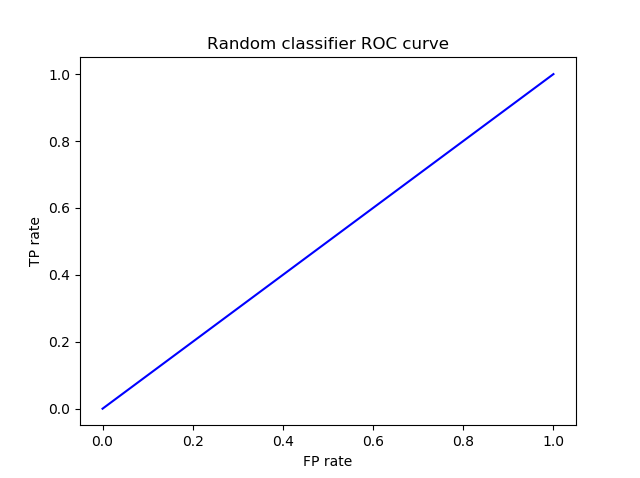
\includegraphics{ex2b}
\\
This is a well known result: a random classifier has a ROC curve that
splits the ROC space in two equal parts.

\subsection{Part c}
Now it is easy to compute the AUC, this ROC curve is a line
following the diagonal of the base square, thus the are under the curve is
half the area of the square.
$$
\text{AUC} = \frac{1}{2}
$$
We could get to the same result using calculus: the underlying function
is $f(x) = x$.
\\
Calculus gives us the formula for the AUC:
$$
\text{AUC} = \int_0^1 f(x) dx
$$
$$
\text{AUC} = \int_0^1 x dx = \left[\frac{x^2}{2} \right]_0^1 
$$
$$
\text{AUC} = \frac{1}{2}
$$

\subsection{Part d}
Having the same error rate on positive and negative examples means having the following:
$$
\frac{\text{FN}}{\text{TP}+\text{FN}} = \frac{\text{FP}}{\text{TN}+\text{FP}}
$$
We compute them by taking only the positive (resp negative) elements from the data
and computing the error rate on this particular set.
Now let's link those two parts to the TP and FP rates. The right part is exactly the expression
of the FP rate. The left one is not exaclty the TP rate:
$$
\frac{\text{FN}}{\text{TP}+\text{FN}} = \frac{\text{TP}+\text{FN} - \text{TP}}{\text{TP}+\text{FN}} = 1 - \frac{\text{TP}}{\text{TP}+\text{FN}}
$$
$$
\frac{\text{FN}}{\text{TP}+\text{FN}} = 1 - \text{TP}_\text{rate}
$$
The first equation now becomes:
$$
1 - \text{TP}_\text{rate} = \text{FP}_\text{rate}
$$
To solve it graphicly, we can slightly change it to the following:
$$
\text{TP}_\text{rate} + \text{FP}_\text{rate} = 1
$$
Now all we have to do is determine all points on the plane whose coordinates add up to one.
This is very easy, it is the line passing through $(0,1)$ and $(1,0)$: the antidiagonal . What we can do is 
draw this line over the ROC curve and the point where both intersect is the point where
the error rate is the same for positive and negative data. 
\\
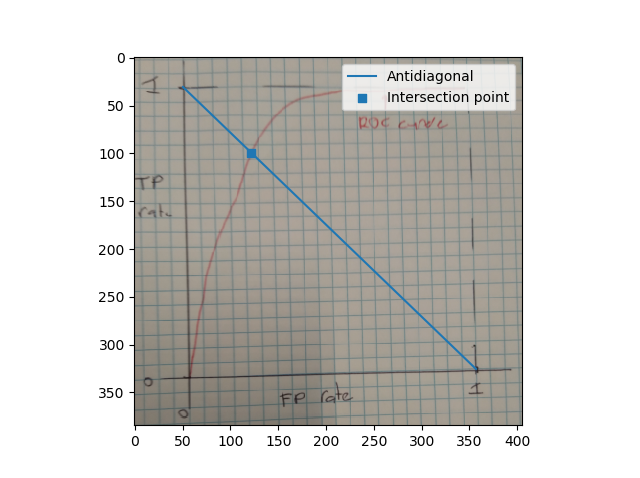
\includegraphics{ex2d}
\\
From this picture, we can now measure the coordinates of the intersection point and the axis with pixel precision.
We get the following result:
$$
\text{P}_\text{intersection} \approx (\text{FP}=0.233, \text{TP}=0.766)
$$
We can check they correctly add up to 1, with little error due to rounding and measure precision.

\section{Exercise 3: Logistic classification \& Regularization}
First let's determine the real label of $x$. We know that the current model misclassfies it,
so if we compute the prediction of the model for $x$, we get the wrong label and thus we can 
deduct the real label.
\\
The easiest way is the compute the quantity $w^\top \bar{x}$, with $\bar{x} = (1,\ x_1,\ x_2,\ x_3)$, and decide its predicted label with the following rule:
$$
\text{Label}_\text{predicted} = \left\{ \begin{array}{ll}  
                                    0 & \text{if $w^\top \bar{x} < 0$}
                                    \\ 
                                    1 & \text{if $w^\top \bar{x} > 0$}
                                        \end{array}
                                \right.
$$
Labels are $0$ and $1$ because we are doing logistic regression and we use the sigmoïd function.
\\
In our case, $w^\top \bar{x} = -1 <0$, thus the predicted label is $0$, and the real label of $x$ is $l=1$.
\subsection{Part a}
First let's apply normal stochastic gradient descent. The formula to update the weights is the following:
$$
w_{new} = w_{old} - \eta \nabla_w E_D(w_{old})
$$
Which gives the following in our case:
$$
w_{new} = w_{old} - \eta (\sigma({w_{old}}^\top \bar{x}) - l) \bar{x}
$$
When we copute this with the values given we obtain the following result which
classifies $x$ accordingly.
$$
w_{new} = \begin{bmatrix}
    0.512, & 1.512, & -2.512, & 0.977
\end{bmatrix}
$$

If we now apply L1 regularization, we need to change our updating formula to the following:
$$
w_{new} = w_{old} - \eta \nabla_w E_D(w_{old}) - \lambda \nabla_w E_w(w_{old})
$$
Where $E_w$ represents an apriori error based on the coordinates of $w$ only. It's purpose
is to introduce error when the coordinates of the discriminant get too big. Doing normalization
should partially prevent our model from over-fitting but not totally.
\\
It is important to not penalyze our model for an important bias (first coordinate): bias is descripted inside the data.
Thus the vector $\nabla_wE_w(w)$ should always have its first coordinate equal to $0$.
\\
In L1 regularization, we define ${E_1}_w(w)$, the order 1 error due to regularization, to be the following:
$$
{E_1}_w(w) = \sum_{i=1}^n \vert w_i \vert
$$
And we can deduce the vector $\nabla_w{E_1}_w(w)$ from this definition:
$$
\nabla_w{E_1}_w(w) = \left(\begin{array}{c}
    0       \\
    h(w_1)  \\
    \vdots  \\
    h(w_n)
\end{array}\right)^\top
$$
Where $h$ is the heaviside function.
\\
We can now compute our new discriminant with L1 regularization based on the previous work:
$$
w_{new} = w_{old} - \eta (\sigma({w_{old}}^\top \bar{x}) - l) \bar{x} - \lambda \left(\begin{array}{c}
                                                                                                0       \\
                                                                                                h({w_{old}}_1)  \\
                                                                                                \vdots  \\
                                                                                                h({w_{old}}_n)
                                                                                            \end{array}\right)^\top
$$
And when we compute the important terms according to the values we obtain the following:
$$
w_{new}^\top \approx \left(\begin{array}{c}
    0  \\
    1  \\
    -2 \\
    2
\end{array}\right) - 0.7 \left(\begin{array}{c}
    -0.731 \\
    -0.731 \\
    0.731  \\
    1.462
\end{array}\right) - 0.2 \left(\begin{array}{c}
    0  \\
    1  \\
    -1 \\
    1
\end{array}\right) \approx
\left(\begin{array}{c}
    0.512 \\
    1.311 \\
    -2.311 \\
    0.776
\end{array}\right)
$$
\subsection{Part b}
Working with L2 regularization instead of L1 will only change $\nabla_wE_w(w)$. This 
is the term relative to the regularization. To determine what we need to put instead of the previous one,
we define the new error due to regularization as follows:
$$
{E_2}_w(w) = \frac{1}{2}\sum_{i=1}^N w_i^2
$$
And its gradient:
$$
\nabla_w{E_2}_w(w) = \left(\begin{array}{c}
    0 \\
    w_1 \\
    \vdots \\
    w_N
\end{array}\right)^\top
$$
We can now replace it in the update equation:
$$
w_{new} = w_{old} - \eta (\sigma({w_{old}}^\top \bar{x}) - l) \bar{x} - \lambda \left(\begin{array}{c}
                                                                                    0 \\
                                                                                    w_1 \\
                                                                                    \vdots \\
                                                                                    w_N
                                                                                \end{array}\right)^\top
$$
$$
w_{new}^\top \approx \left(\begin{array}{c}
    0  \\
    1  \\
    -2 \\
    2
\end{array}\right) - 0.7 \left(\begin{array}{c}
    -0.731 \\
    -0.731 \\
    0.731  \\
    1.462
\end{array}\right) - 0.2 \left(\begin{array}{c}
    0  \\
    1  \\
    -1 \\
    1
\end{array}\right) \approx
\left(\begin{array}{c}
    0.512 \\
    1.311 \\
    -2.111 \\
    0.576
\end{array}\right)
$$

\section{Exercise 4: MCQ}
In the following MCQs, a $\diamondsuit$ signifies this proposition is part of the right answer.
\subsection{MCQ 1}
This question verifies if the student understood correctly how to compute the recall
\\
Q: Given the following confusion matrix, compute the recall of B. Rounded up to 2 decimals.
\begin{center}
    \begin{tabular}{ |c|c|c| }
        \hline
        Actual $\backslash$ Predicted & A & B \\
        \hline
        A & $ 314 $ & $ 159 $ \\
        B & $ 265 $ & $ 358 $ \\
        \hline
    \end{tabular}
\end{center}
\begin{enumerate}
    \item $0.34$
    \item $0.57$
    \item $0.66$
    \item $0.69$ $\diamondsuit$
\end{enumerate}

\subsection{MCQ 2}
This question checks if the student understands how to interpret a ROC curve and can compare
classifier based on their respective ROC curves.
\\
Q: Which of these classifiers is (are) better than a random classifier ? 
\\
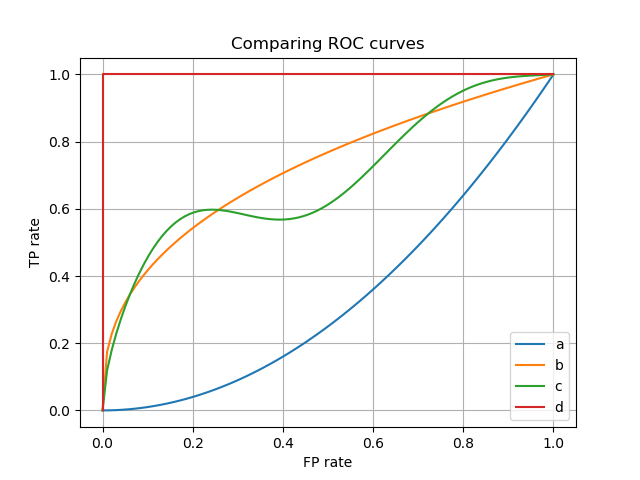
\includegraphics{ex4}
\\
\begin{enumerate}
    \item a
    \item b $\diamondsuit$
    \item c $\diamondsuit$
    \item d $\diamondsuit$
\end{enumerate}
\end{document}
